\documentclass[11pt,a4paper]{article}
\usepackage[margin=20mm,headheight=14pt]{geometry}
\usepackage[T1]{fontenc}
\usepackage{lmodern,microtype}
\usepackage{graphicx,xcolor,booktabs,tabularx,array,enumitem,tikz,fancyhdr,hyperref}
\usetikzlibrary{arrows.meta,positioning}
\definecolor{ink}{HTML}{182536}
\definecolor{muted}{HTML}{526174}
\definecolor{teal}{HTML}{087F75}
\definecolor{pale}{HTML}{EAF5F3}
\definecolor{line}{HTML}{C8D2DC}
\definecolor{blue}{HTML}{245EA8}
\definecolor{amber}{HTML}{9A6410}
\hypersetup{colorlinks=true,linkcolor=teal,urlcolor=blue,pdftitle={What Changed in the Room: Architecture and Design Rationale},pdfauthor={What Changed in the Room project}}
\setlength{\parindent}{0pt}\setlength{\parskip}{5pt}
\setlist[itemize]{leftmargin=1.4em,itemsep=2pt,topsep=2pt}
\renewcommand{\arraystretch}{1.18}
\pagestyle{fancy}\fancyhf{}
\fancyhead[L]{\small\color{muted}WHAT CHANGED IN THE ROOM}
\fancyhead[R]{\small\color{muted}DESIGN NOTE}
\fancyfoot[C]{\small\color{muted}\thepage}
\renewcommand{\headrulewidth}{0.4pt}
\newcommand{\imagepanel}[3]{%
\fcolorbox{line}{white}{\begin{minipage}[c][#3][c]{#2}\centering
\IfFileExists{figures/#1}{\includegraphics[width=\linewidth,height=0.78#3,keepaspectratio]{figures/#1}}{%
{\color{teal}\bfseries IMAGE SLOT}\\[4pt]
{\small\color{muted}Add \texttt{\detokenize{docs/figures/#1}} and recompile.}}\end{minipage}}}
\begin{document}
\thispagestyle{empty}
\vspace*{3mm}
{\large\color{teal}\textbf{SYSTEM DESIGN NOTE}}\\[4mm]
{\Huge\bfseries\color{ink}What Changed in the Room?}\\[2mm]
{\large\color{muted}Architecture and design rationale for comparing two indoor phone recordings}
\vspace{5mm}

\fcolorbox{teal}{pale}{\begin{minipage}{0.95\linewidth}
\textbf{CPU-capable by design.} No NVIDIA GPU or CUDA installation is required. The workflow uses COLMAP's sparse CPU reconstruction, compact perception models, and OpenMVS's CPU reconstruction tools. A GPU can speed up neural inference, but remains optional. The tradeoff is longer processing time, especially for OpenMVS depth estimation and fusion when producing colored room maps.
\end{minipage}}

\vspace{4mm}
{\Large\bfseries\color{ink}Architecture at a glance}
\vspace{2mm}

\begin{center}
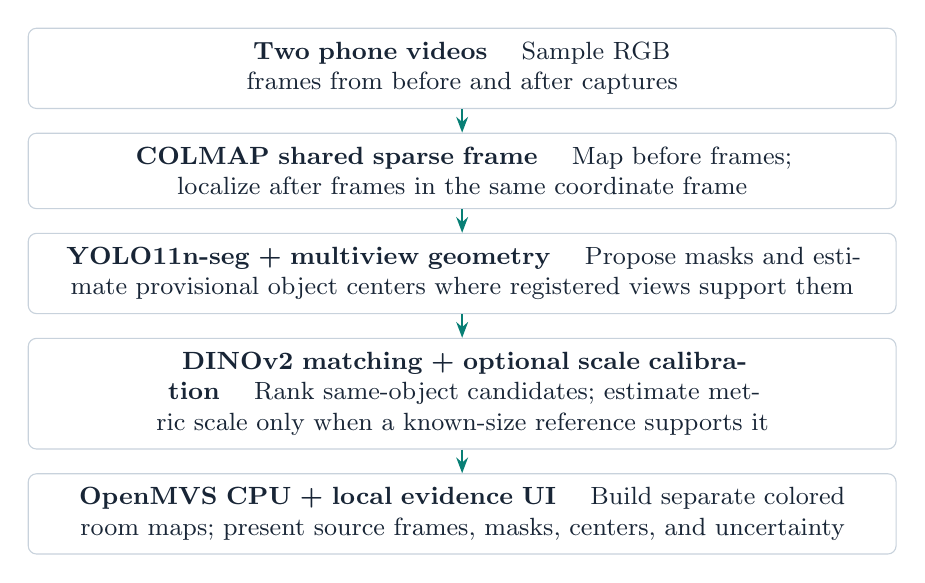
\begin{tikzpicture}[
 block/.style={draw=line,rounded corners=3pt,fill=white,text=ink,align=center,text width=0.88\textwidth,inner sep=5pt,font=\small},
 arrow/.style={-{Stealth[length=2mm]},line width=0.8pt,draw=teal}
]
\node[block] (input) {\textbf{Two phone videos} \quad Sample RGB frames from before and after captures};
\node[block,below=3mm of input] (map) {\textbf{COLMAP shared sparse frame} \quad Map before frames; localize after frames in the same coordinate frame};
\node[block,below=3mm of map] (objects) {\textbf{YOLO11n-seg + multiview geometry} \quad Propose masks and estimate provisional object centers where registered views support them};
\node[block,below=3mm of objects] (match) {\textbf{DINOv2 matching + optional scale calibration} \quad Rank same-object candidates; estimate metric scale only when a known-size reference supports it};
\node[block,below=3mm of match] (maps) {\textbf{OpenMVS CPU + local evidence UI} \quad Build separate colored room maps; present source frames, masks, centers, and uncertainty};
\draw[arrow] (input)--(map); \draw[arrow] (map)--(objects); \draw[arrow] (objects)--(match); \draw[arrow] (match)--(maps);
\end{tikzpicture}
\end{center}

\textbf{Objective.} Align two recordings of the same room, identify candidate object changes, and show the evidence needed to assess them. This is an offline review system, not a complete digital twin or a validated autonomous-navigation system. The colored maps are for visual communication; change positions come from the shared COLMAP frame.

\vfill
{\small\color{muted}System components are intentionally separated so that camera alignment, object appearance, provisional geometry, and visual reconstruction can each be inspected.}
\newpage

\section*{Architecture and component choices}

The system samples RGB frames from both videos. COLMAP reconstructs a sparse reference from the before frames and registers after frames into that reference when overlap and texture permit. This shared coordinate frame is necessary because independent monocular reconstructions have unrelated poses and scales.

YOLO11n-seg proposes common object classes and instance masks. Registered multiview observations support provisional 3D object centers. Depth Anything V2 Small supplies relative depth for selected views; the depth is fit to COLMAP camera-depth observations before geometric use. The current UI assumes reference TV dimensions of 0.90 × 0.55 m to estimate a provisional, per-recording meters-per-map-unit scale. If the TV differs, that estimate may be wrong; the dimensions are fixed in code rather than exposed as UI controls.

DINOv2 ViT-S/14 compares masked object crops across recordings. Appearance similarity is combined with labels and supported 3D anchors to rank possible same-object pairs. It does not create persistent identities or prove that two detections are the same physical object.

OpenMVS receives shared camera poses and the RGB frames, then estimates and fuses depth maps to make separate before and after textured surfaces. This CPU multiview-stereo step is distinct from COLMAP sparse mapping. It improves human inspection; it is not the source of change geometry.

\vspace{1mm}
\begin{tabularx}{\linewidth}{@{}>{\raggedright\arraybackslash}p{0.18\linewidth}XX@{}}
\toprule
\textbf{Component} & \textbf{Purpose / rationale} & \textbf{Tradeoff / boundary} \\
\midrule
COLMAP sparse SfM & Camera poses and common reference; CPU feature extraction and matching. & Incomplete landmarks, arbitrary scale, overlap-sensitive registration. \\
YOLO11n-seg & Compact model for common-object labels and masks. & Closed-set classes; small, unusual, occluded, or blurred objects may be missed. \\
DINOv2 ViT-S/14 & Visual embeddings rank cross-capture crop similarity. & Similarity is heuristic; similar instances and viewpoint changes can confuse it. \\
Depth Anything V2 Small & Relative-depth cue that can be calibrated against COLMAP and a known object. & Not metric by itself; sparse or biased anchors can invalidate scale. \\
OpenMVS CPU & Colored room surfaces make captures easier to interpret. & Depth estimation and fusion are the heaviest stage; holes and artifacts are possible. \\
Streamlit UI & Local upload, processing, evidence review, and map presentation. & Offline batch workflow; first model use needs downloads unless weights are cached. \\
\bottomrule
\end{tabularx}

\vspace{2mm}
\textbf{Why this stack is lightweight.} It favors sparse mapping and compact model variants over GPU-only reconstruction and large end-to-end VLMs. That reduces accelerator requirements and keeps the evidence stages inspectable. CPU capability does not mean real-time speed or low memory use for every input; OpenMVS is expected to take the most time.

\newpage
\section*{Evidence, claim boundaries, and limitations}

\textbf{Moved object.} A movement candidate needs a plausible same-object association and supported before/after centers in the shared frame. Review the source frames and masks. Report meters only if this recording's known-object calibration passes; otherwise use map units.

\textbf{Added or removed object.} An unmatched detection is a candidate, not a conclusion. A detector miss, unregistered frame, or missing sparse point is never proof of removal. The expected region must be visibly covered and empty across useful after views; occlusion and incomplete coverage remain alternatives.

\begin{itemize}
\item Camera motion, blur, exposure changes, repeated textures, and low overlap can prevent registration.
\item Centers are approximate anchors, not object surfaces; mask errors, partial views, and occlusion affect them.
\item DINOv2 can confuse similar instances. Current similarity thresholds are demo heuristics, not validated accuracy.
\item Metric scale is provisional, assumes the TV is 0.90 × 0.55 m, and is not survey-grade. A differently sized TV can bias the reported scale.
\item OpenMVS surfaces may be incomplete; differences can reflect capture coverage as well as scene changes.
\item The system is for offline analysis, not real-time robot control or a safety guarantee.
\end{itemize}

\vspace{2mm}
\begin{minipage}[t]{0.48\linewidth}
\textbf{Segmentation example}\\[-1mm]
\small\color{muted}Use a real before/after frame pair with YOLO masks and labels.\\[2mm]
\imagepanel{segmentation_example.png}{0.95\linewidth}{44mm}
\end{minipage}\hfill
\begin{minipage}[t]{0.48\linewidth}
\textbf{Paired RGB room maps}\\[-1mm]
\small\color{muted}Use the paired map view from a representative run.\\[2mm]
\imagepanel{paired_room_maps.png}{0.95\linewidth}{44mm}
\end{minipage}

\vspace{4mm}
\textbf{Object-change evidence}\\[-1mm]
\small\color{muted}Show source frames, masks, old/new centers, and uncertainty for one moved or possibly removed object. Do not present a detector miss alone as confirmed removal.\\[2mm]
\imagepanel{change_evidence.png}{0.96\linewidth}{35mm}

\vfill
{\footnotesize\color{muted}Setup and launch steps are in the README. COLMAP and OpenMVS are native dependencies; models download on first use. Videos, weights, and generated runs are not included by default.}
\end{document}
